\section{Construcción de un Pipeline Parametrizado}
\label{sec:arquitectura}

El desarrollo de un sistema de predicción clínica basado en aprendizaje automático requiere una infraestructura de software que facilite la experimentación, garantice la reproducibilidad y permita la escalabilidad del proceso investigativo. En esta sección se expone el diseño de la arquitectura implementada para soportar los experimentos descritos previamente de una manera organizada.

El enfoque de este proyecto se fundamenta en la premisa de que la construcción de un sistema predictivo robusto requiere un estudio exploratorio sistemático. Antes de automatizar un flujo de producción, es necesario experimentar con múltiples configuraciones, algoritmos y combinaciones de características para identificar qué funciona mejor en el dominio específico de la predicción de shock hemorrágico. Por esta razón, el proyecto se diseñó como una propuesta hacia la automatización: un pipeline parametrizado que permite al investigador definir experimentos de forma declarativa, ejecutar múltiples configuraciones sin modificar código, y comparar resultados de manera sistemática.

Este enfoque de parametrización es particularmente relevante en el contexto clínico, donde las decisiones de modelado deben ser trazables, reproducibles y auditables. La metodología de experimentación sistemática (cinco experimentos secuenciales: baseline, agregaciones, categorizaciones, pruning e hiperparámetros) valida la necesidad de este diseño modular y configurable.

\subsection{Evaluación de plataformas de procesamiento}

Para llevar a cabo el procesamiento de los datos clínicos y la transformación de características, se consideró inicialmente el uso de tecnologías de Big Data como Apache Spark. Sin embargo, al analizar el volumen real de la información tabular disponible, se evidenció que su magnitud permitía un manejo eficiente directamente en la memoria del sistema. Incorporar una plataforma de procesamiento distribuido habría sumando una complejidad técnica en su configuración y mantenimiento que no estaba justificada para las necesidades del proyecto. Por esta razón, se prefirió un enfoque apoyado en librerías estándar de Python. Esta decisión facilitó el desarrollo y permitió mantener el flujo de trabajo funcional sin requerir infraestructura computacional adicional.

\subsection{Control de la escalabilidad en la experimentación}

Al adoptar un entorno basado en rutinas de Python, apareció la necesidad de organizar adecuadamente la fase de experimentación. Durante el modelado es frecuente que, al probar la inclusión de nuevas variables o ajustar parámetros, se acumulen fragmentos de código repetidos o se incluyan valores estáticos directamente en los archivos principales.

En este trabajo, la escalabilidad técnica se entiende como la capacidad de ampliar los experimentos —añadiendo nuevos algoritmos o ajustando los existentes— sin alterar el código base. Abordar este problema fue fundamental para prevenir errores accidentales y proteger la estabilidad lógica de los flujos que ya habían sido verificados. El diseño del pipeline parametrizado responde directamente a esta necesidad: cada experimento puede ejecutarse con una configuración diferente sin necesidad de modificar los scripts de entrenamiento o evaluación.

\subsection{Orquestación y reproducibilidad mediante Apache Airflow}

Con la intención de dar estructura al flujo de ejecución y evitar el lanzamiento manual de tareas, se integró Apache Airflow como orquestador. Las rutinas de limpieza de datos, extracción de características, entrenamiento y evaluación fueron modeladas a través de Grafos Acíclicos Dirigidos (DAGs). Al delegar el control del proceso a un orquestador, se automatiza la resolución de dependencias entre cada paso del proceso. Esto consolida un sistema más tolerante a errores interrupciones y garantiza que la ejecución de los experimentos reportados en este documento sea replicable de manera exacta e independiente.

\subsection{Desacoplamiento mediante el patrón Factory y archivos YAML}

Una vez establecido el orden de ejecución con Airflow, resultó necesario separar la programación de la definición de los modelos predictivos. Para ello, se implementó el patrón de diseño \textit{Factory}, el cual trabaja en conjunto con un administrador de configuraciones centralizado (\texttt{ConfigurationManager} en \texttt{src/utils/config\_manager.py}) que consume archivos en formato YAML (\texttt{pipeline\_config.yaml}).

A nivel estructural, la configuración de un modelo se consolida mediante secciones jerárquicas y autodescriptivas. En el archivo YAML se define un bloque específico para cada estimador, indicando la ruta de la librería base (el módulo fuente), el nombre exacto de la clase del algoritmo y un diccionario con los hiperparámetros que regirán su entrenamiento. Un ejemplo simplificado de esta estructura es el siguiente:

\begin{verbatim}
models:
  random_forest:
    module: "sklearn.ensemble"
    class: "RandomForestClassifier"
    params:
      n_estimators: 100
      max_depth: 10
      random_state: 42
\end{verbatim}

Esta aproximación permite que los detalles de cada experimento se definan de forma completamente declarativa. Por ejemplo, al procesar el fragmento YAML anterior, el componente \textit{Factory} centralizado en el archivo \texttt{src/models/train.py} (a través de su función \texttt{get\_model\_from\_config}) lee las propiedades \texttt{module} y \texttt{class} del archivo de texto. Posteriormente, utilizando la librería nativa \texttt{importlib.import\_module()}, el sistema instancia el estimador de manera automatizada y le transfiere sus parámetros correspondientes. A continuación, el sistema construye el \textit{pipeline} definitivo (\texttt{create\_pipeline()}) añadiendo los preprocesamientos requeridos, como la estandarización de los datos numéricos o la poda de características. Gracias a esto, cambiar de un clasificador Random Forest a un XGBoost, o alterar la profundidad máxima de un árbol, se resuelve editando unas cuantas líneas en un archivo de texto, sin necesidad de intervenir la base del método \texttt{train\_model()}. Esto aísla la complejidad técnica y permite la organización de múltiples pruebas experimentales de forma limpia, sistemática y auditable.

\subsection{Organización de reportes y resultados}

La facilidad para plantear nuevas pruebas incremento paralelamente la generación de resultados analíticos, abarcando gráficas de desempeño (curvas ROC), métricas numéricas y resúmenes de importancia de variables.

Para asegurar un manejo ordenado de estos documentos y evitar que la información de distintos experimentos se entrelace, la arquitectura incorpora un módulo encargado de clasificar automáticamente los archivos resultantes. Terminada cada ejecución, el sistema organiza las gráficas y reportes en carpetas estructuradas según el identificador del experimento y el algoritmo evaluado. Esto facilita la consulta de la información y estandariza la recolección de resultados.

\subsection{Interfaz de usuario para la validación de configuraciones}

El componente final de la arquitectura consiste en una interfaz de usuario diseñada para facilitar la construcción de los archivos YAML. Dado que la redacción manual de código en texto plano hace habitual la aparición de errores en la indentación o en la escritura de los parámetros, esta herramienta gráfica valida que la configuración ingresada cumpla con el formato esperado antes de que el experimento se inicie.

La aplicación, desarrollada en Streamlit, permite al investigador configurar todos los aspectos del pipeline mediante una interfaz visual e intuitiva. A continuación se describe la estructura y funcionalidad de cada sección de la interfaz.

\subsection{Descripción de la interfaz Streamlit}

La interfaz del editor de configuración se estructura en diez secciones principales, accesibles desde la barra de navegación lateral. Cada sección corresponde a un componente específico del pipeline y permite su configuración de forma aislada.

La \textbf{sección de configuración general} permite al usuario definir parámetros globales del pipeline, tales como la versión del pipeline, la versión del dataset y la semilla aleatoria para reproducibilidad. También incluye opciones de visualización para las gráficas generadas (resolución DPI). Estos parámetros aseguran la trazabilidad experimental: la versión del pipeline controla las rutas de salida de modelos y resultados, mientras que la semilla aleatoria garantiza la reproducibilidad de los experimentos, aspecto fundamental en investigación científica.

\begin{figure}[H]
\centering
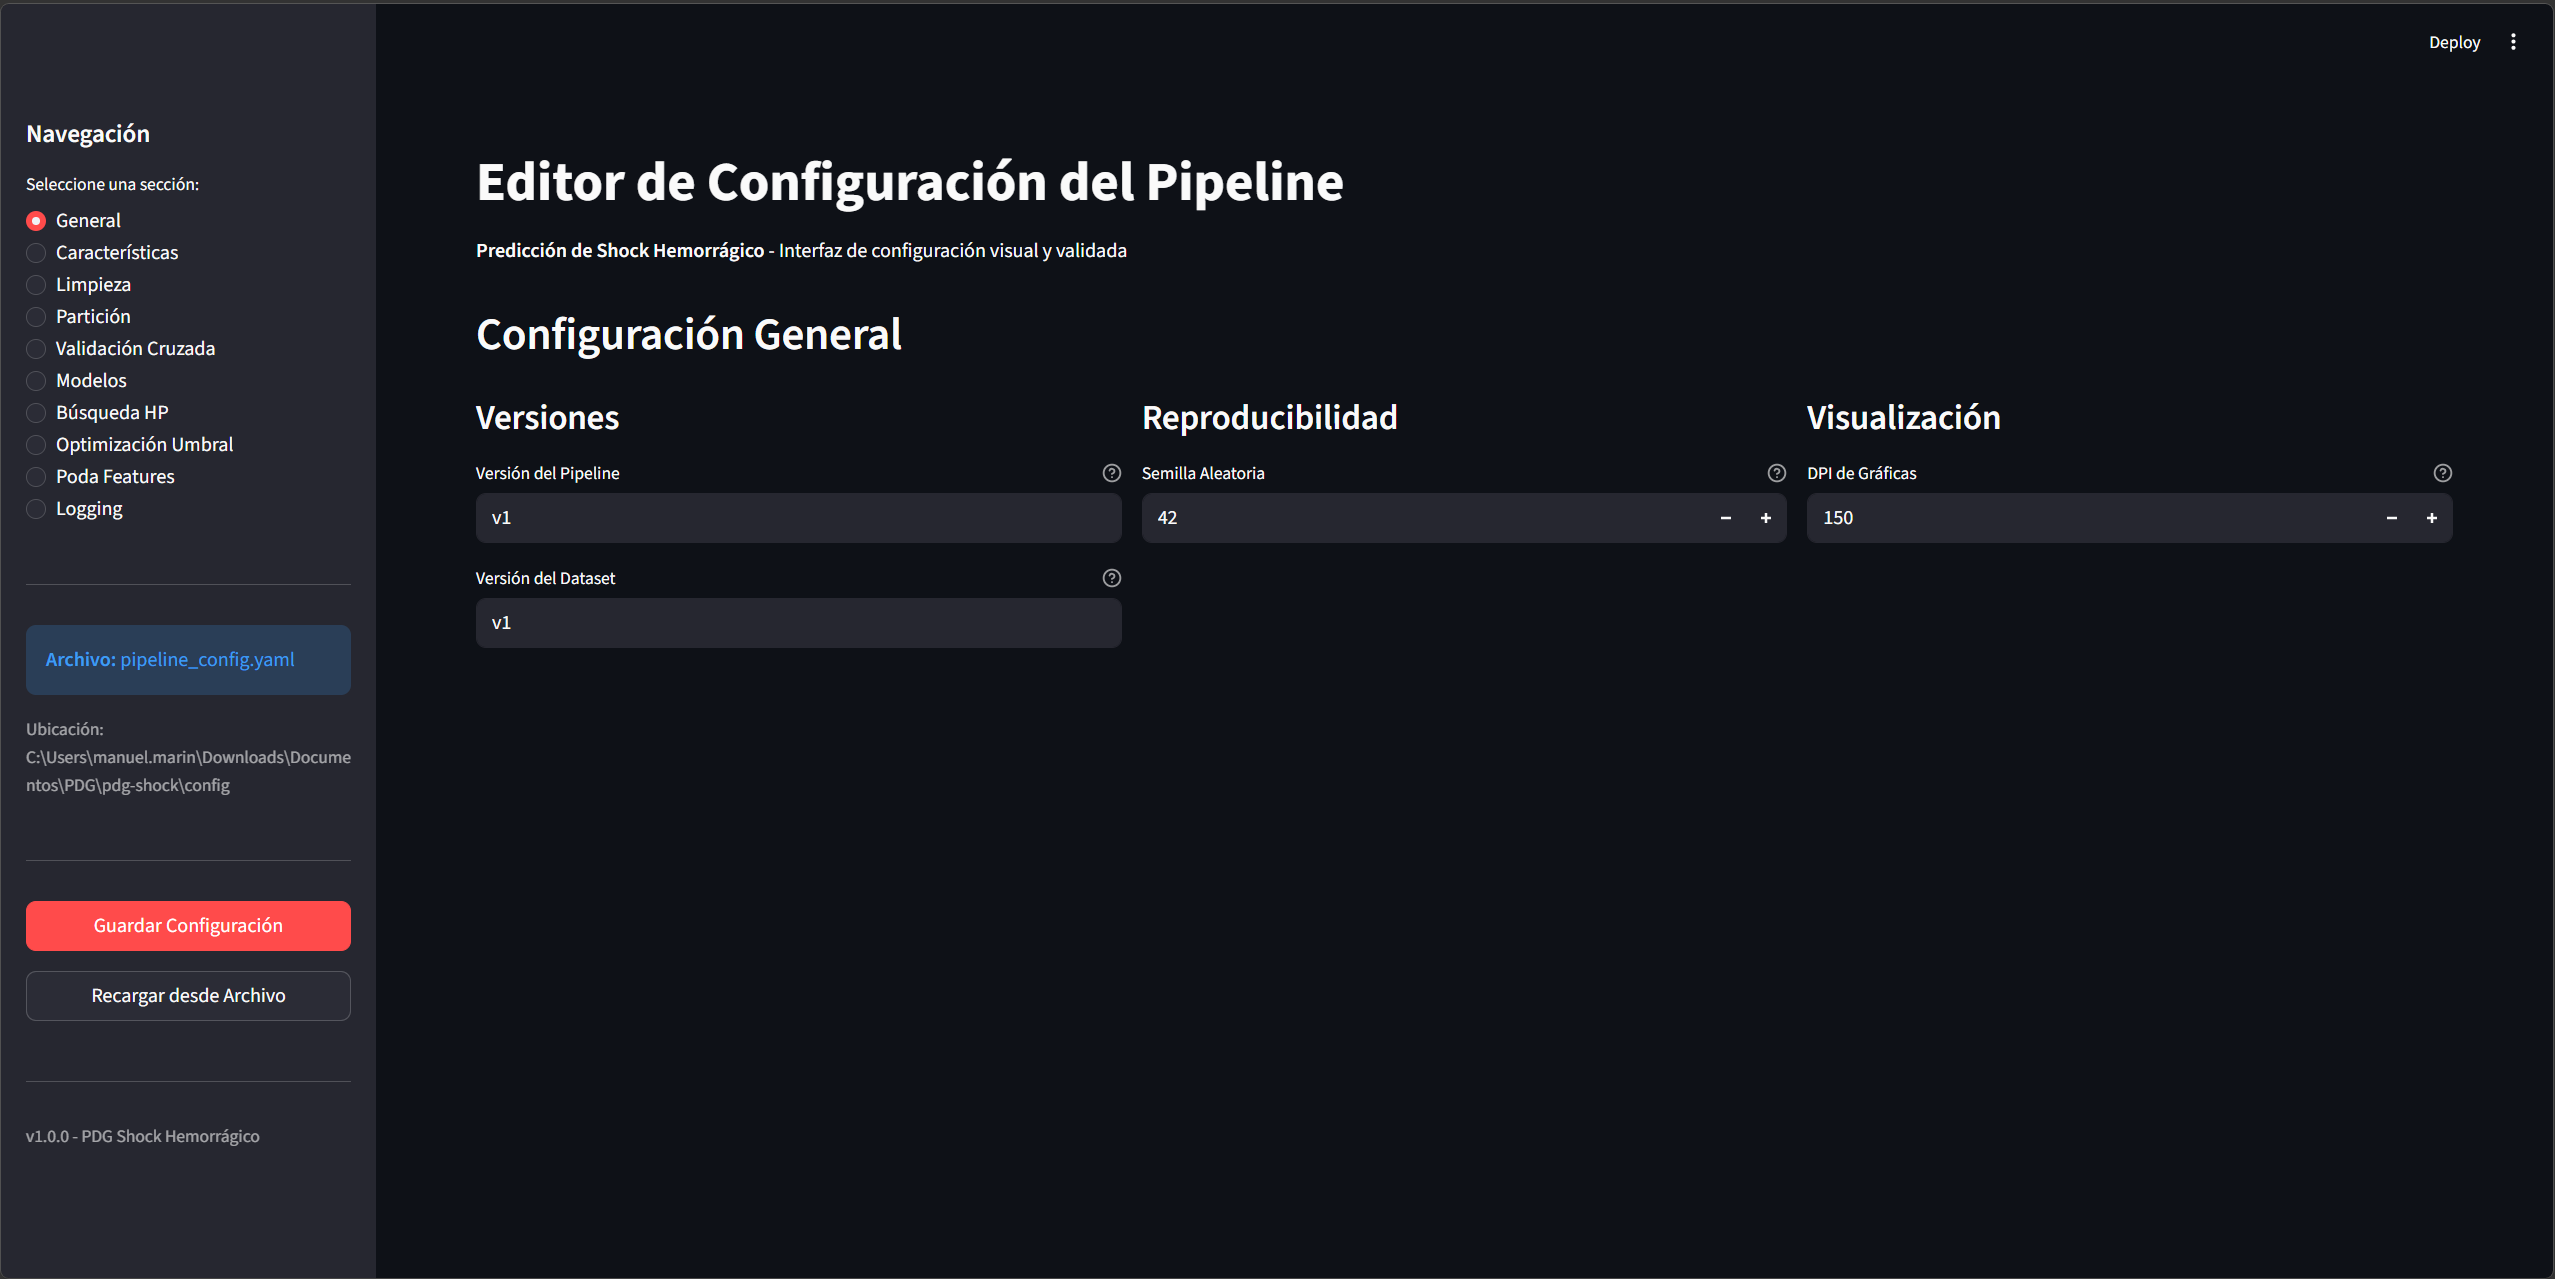
\includegraphics[width=0.85\textwidth]{images/editor_general.png}
\caption{Vista general del editor de configuración del pipeline. La interfaz permite modificar parámetros generales como versiones, semilla aleatoria y opciones de visualización.}
\label{fig:editor-general}
\end{figure}

La \textbf{sección de características} permite gestionar las variables del modelo (Figura \ref{fig:editor-caracteristicas}). Incluye la definición de la variable objetivo (SHOCK), las características numéricas (EDAD, HB\_PREQX), binarias (comorbilidades como DIABETES, HIPERTENSION), agregadas (definidas mediante operaciones aritméticas sobre otras variables) y categóricas (discretizaciones de variables continuas). Para las features agregadas y categóricas, el usuario puede habilitarlas o deshabilitarlas individualmente mediante expandibles, permitiendo un control granular sobre qué variables se incluyen en cada experimento. Los tipos de agregación disponibles son: suma, producto e inverso binario. Las features categóricas se configuran mediante umbrales sobre variables fuente.

\begin{figure}[H]
\centering
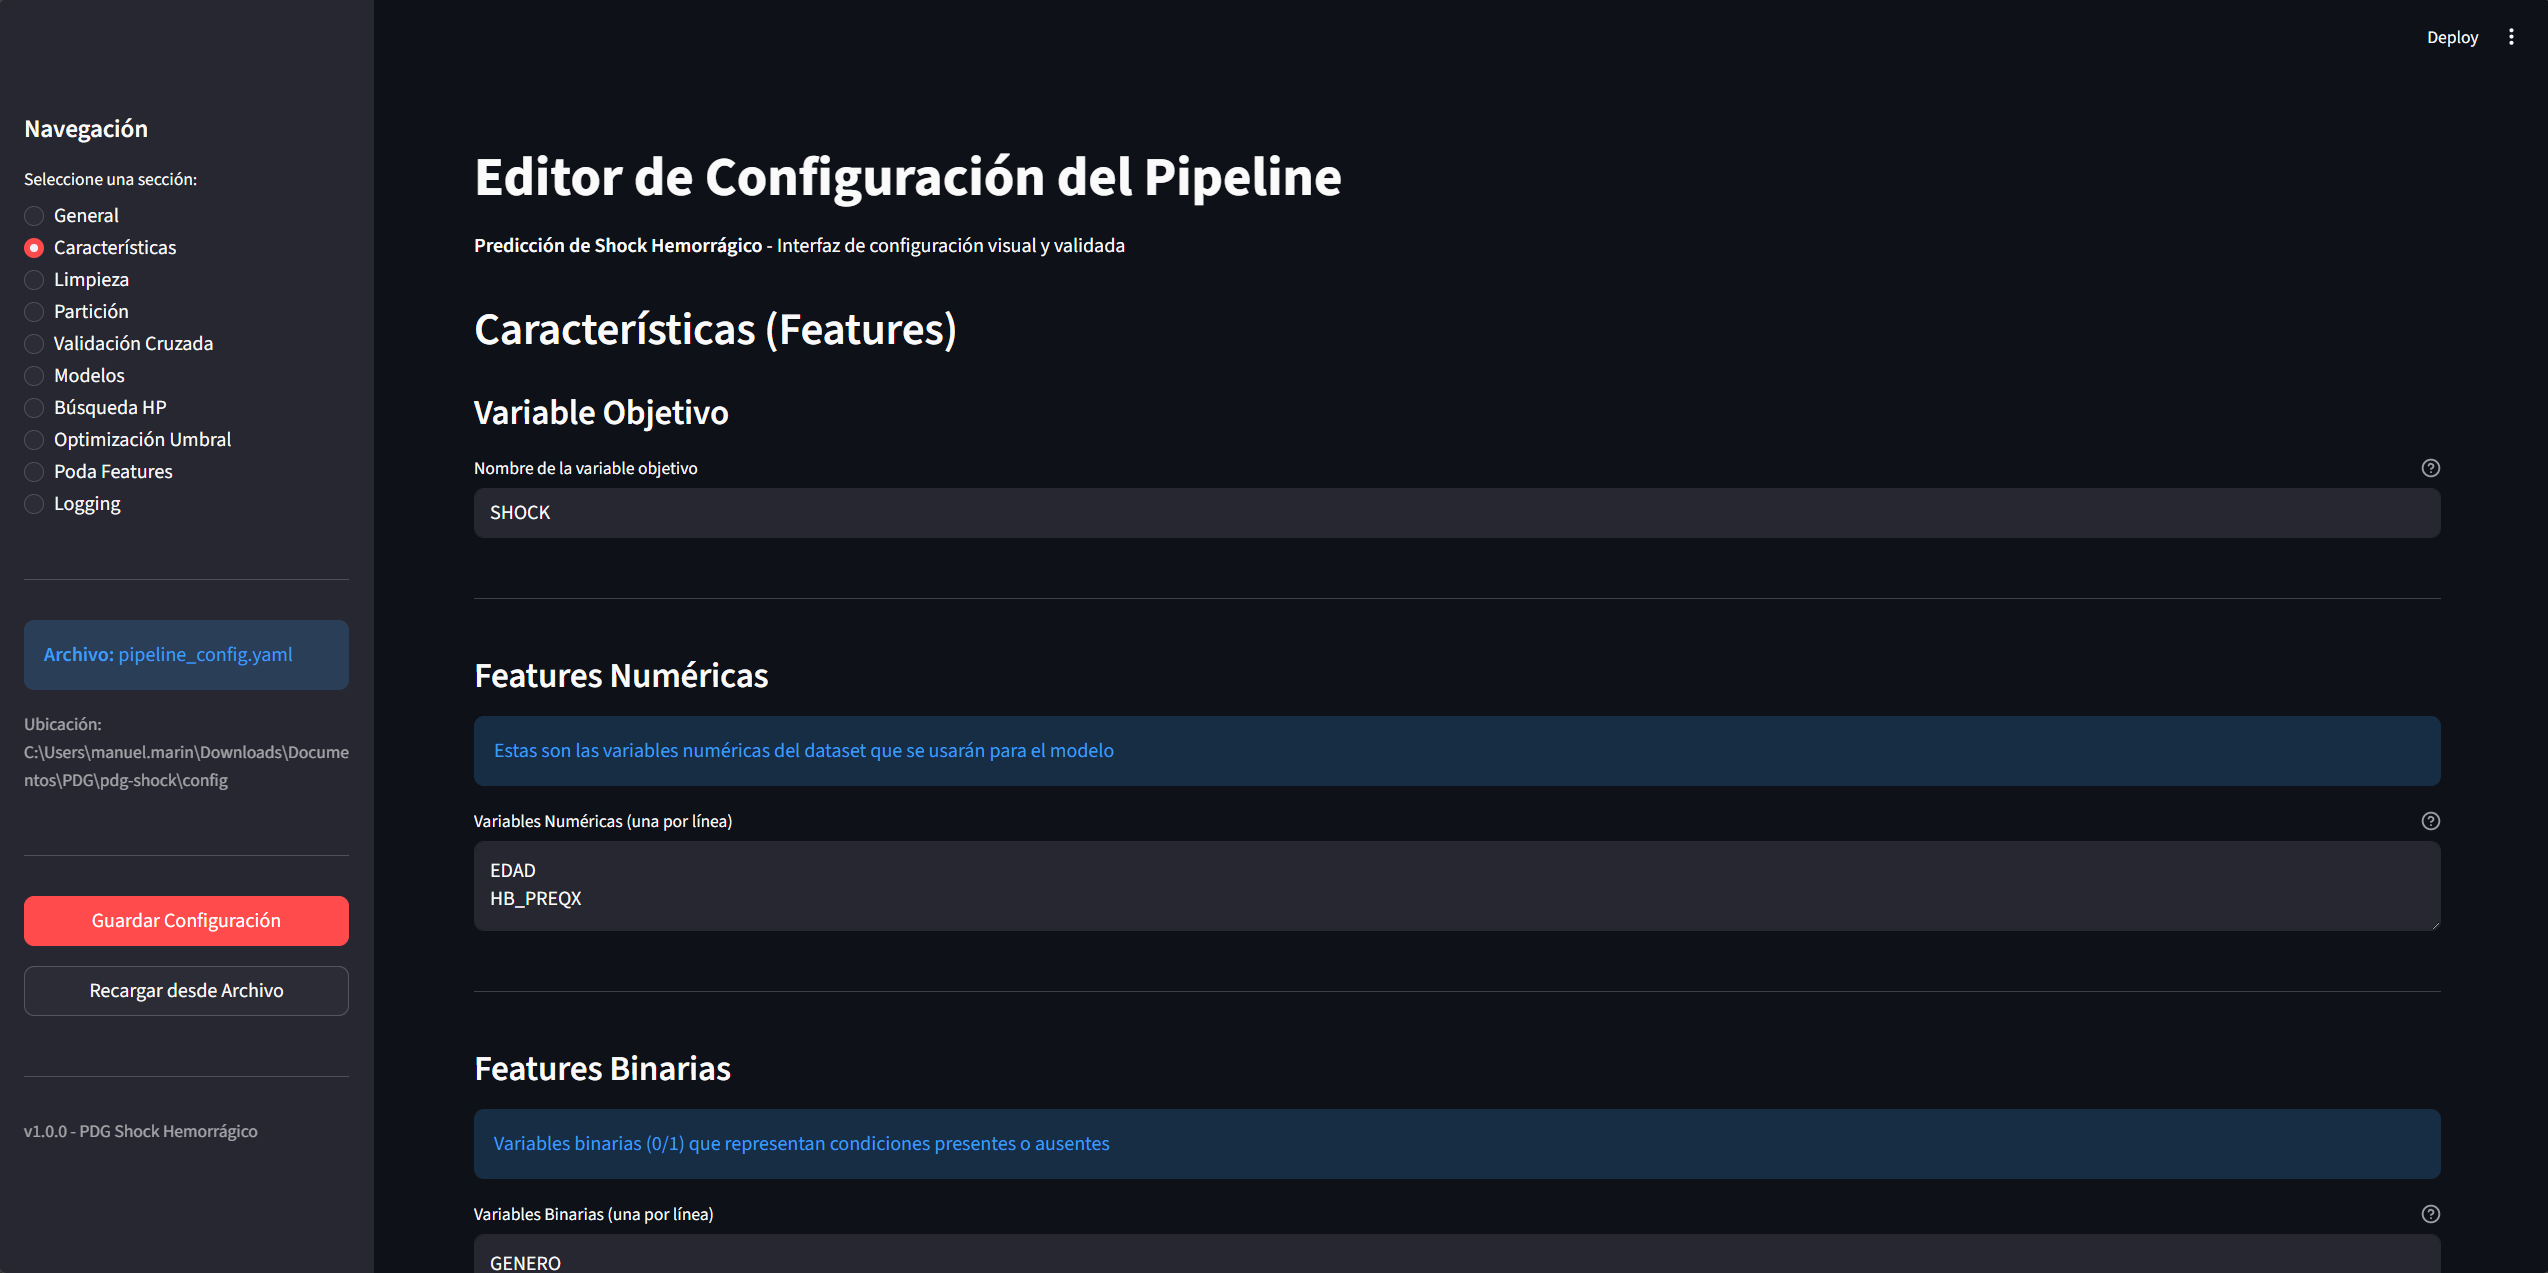
\includegraphics[width=0.85\textwidth]{images/editor_caracteristicas.png}
\caption{Sección de configuración de características. Permite definir la variable objetivo, features numéricas, binarias, agregadas y categóricas.}
\label{fig:editor-caracteristicas}
\end{figure}

La \textbf{sección de limpieza y validación de datos} permite al investigador definir reglas de calidad de datos. Incluye la especificación de columnas a excluir del dataset (como identificadores o datos de fuga), la validación de valores binarios permitidos (0 o 1) y la definición de rangos válidos para variables críticas como EDAD (mínimo y máximo) y HB\_PREQX (hemoglobina prequirúrgica en g/dL). La interfaz incorpora validadores automáticos que verifican que los rangos ingresados sean coherentes, rejectando configuraciones inválidas como valores negativos de edad o valores de hemoglobina fuera del rango fisiológico plausible (0-30 g/dL).

La \textbf{sección de partición de datos (Train/Test Split)} gestiona la división del dataset para entrenamiento y evaluación. Permite configurar la proporción del conjunto de prueba (slider entre 10\% y 50\%), activar la mezcla aleatoria de datos (shuffle) y habilitar la partición estratificada para mantener la proporción de clases en train y test. La estratificación es especialmente importante en datasets desbalanceados como el del presente estudio, donde la proporción de casos de shock es menor que la de no-shock. La interfaz muestra en tiempo real la distribución resultante (ej: 80\% train, 20\% test) según la selección del usuario.

La \textbf{sección de validación cruzada} configura los parámetros de la evaluación mediante k-fold cross-validation. El investigador puede especificar el número de folds (entre 2 y 20), activar el escalamiento de features (normalización de variables numéricas, recomendada) y configurar el procesamiento paralelo (número de cores, con valor -1 para utilizar todos los disponibles). La validación cruzada estratificada garantiza que cada fold mantenga la proporción de la variable objetivo, proporcionando estimaciones más estables del rendimiento del modelo.

\begin{figure}[H]
\centering
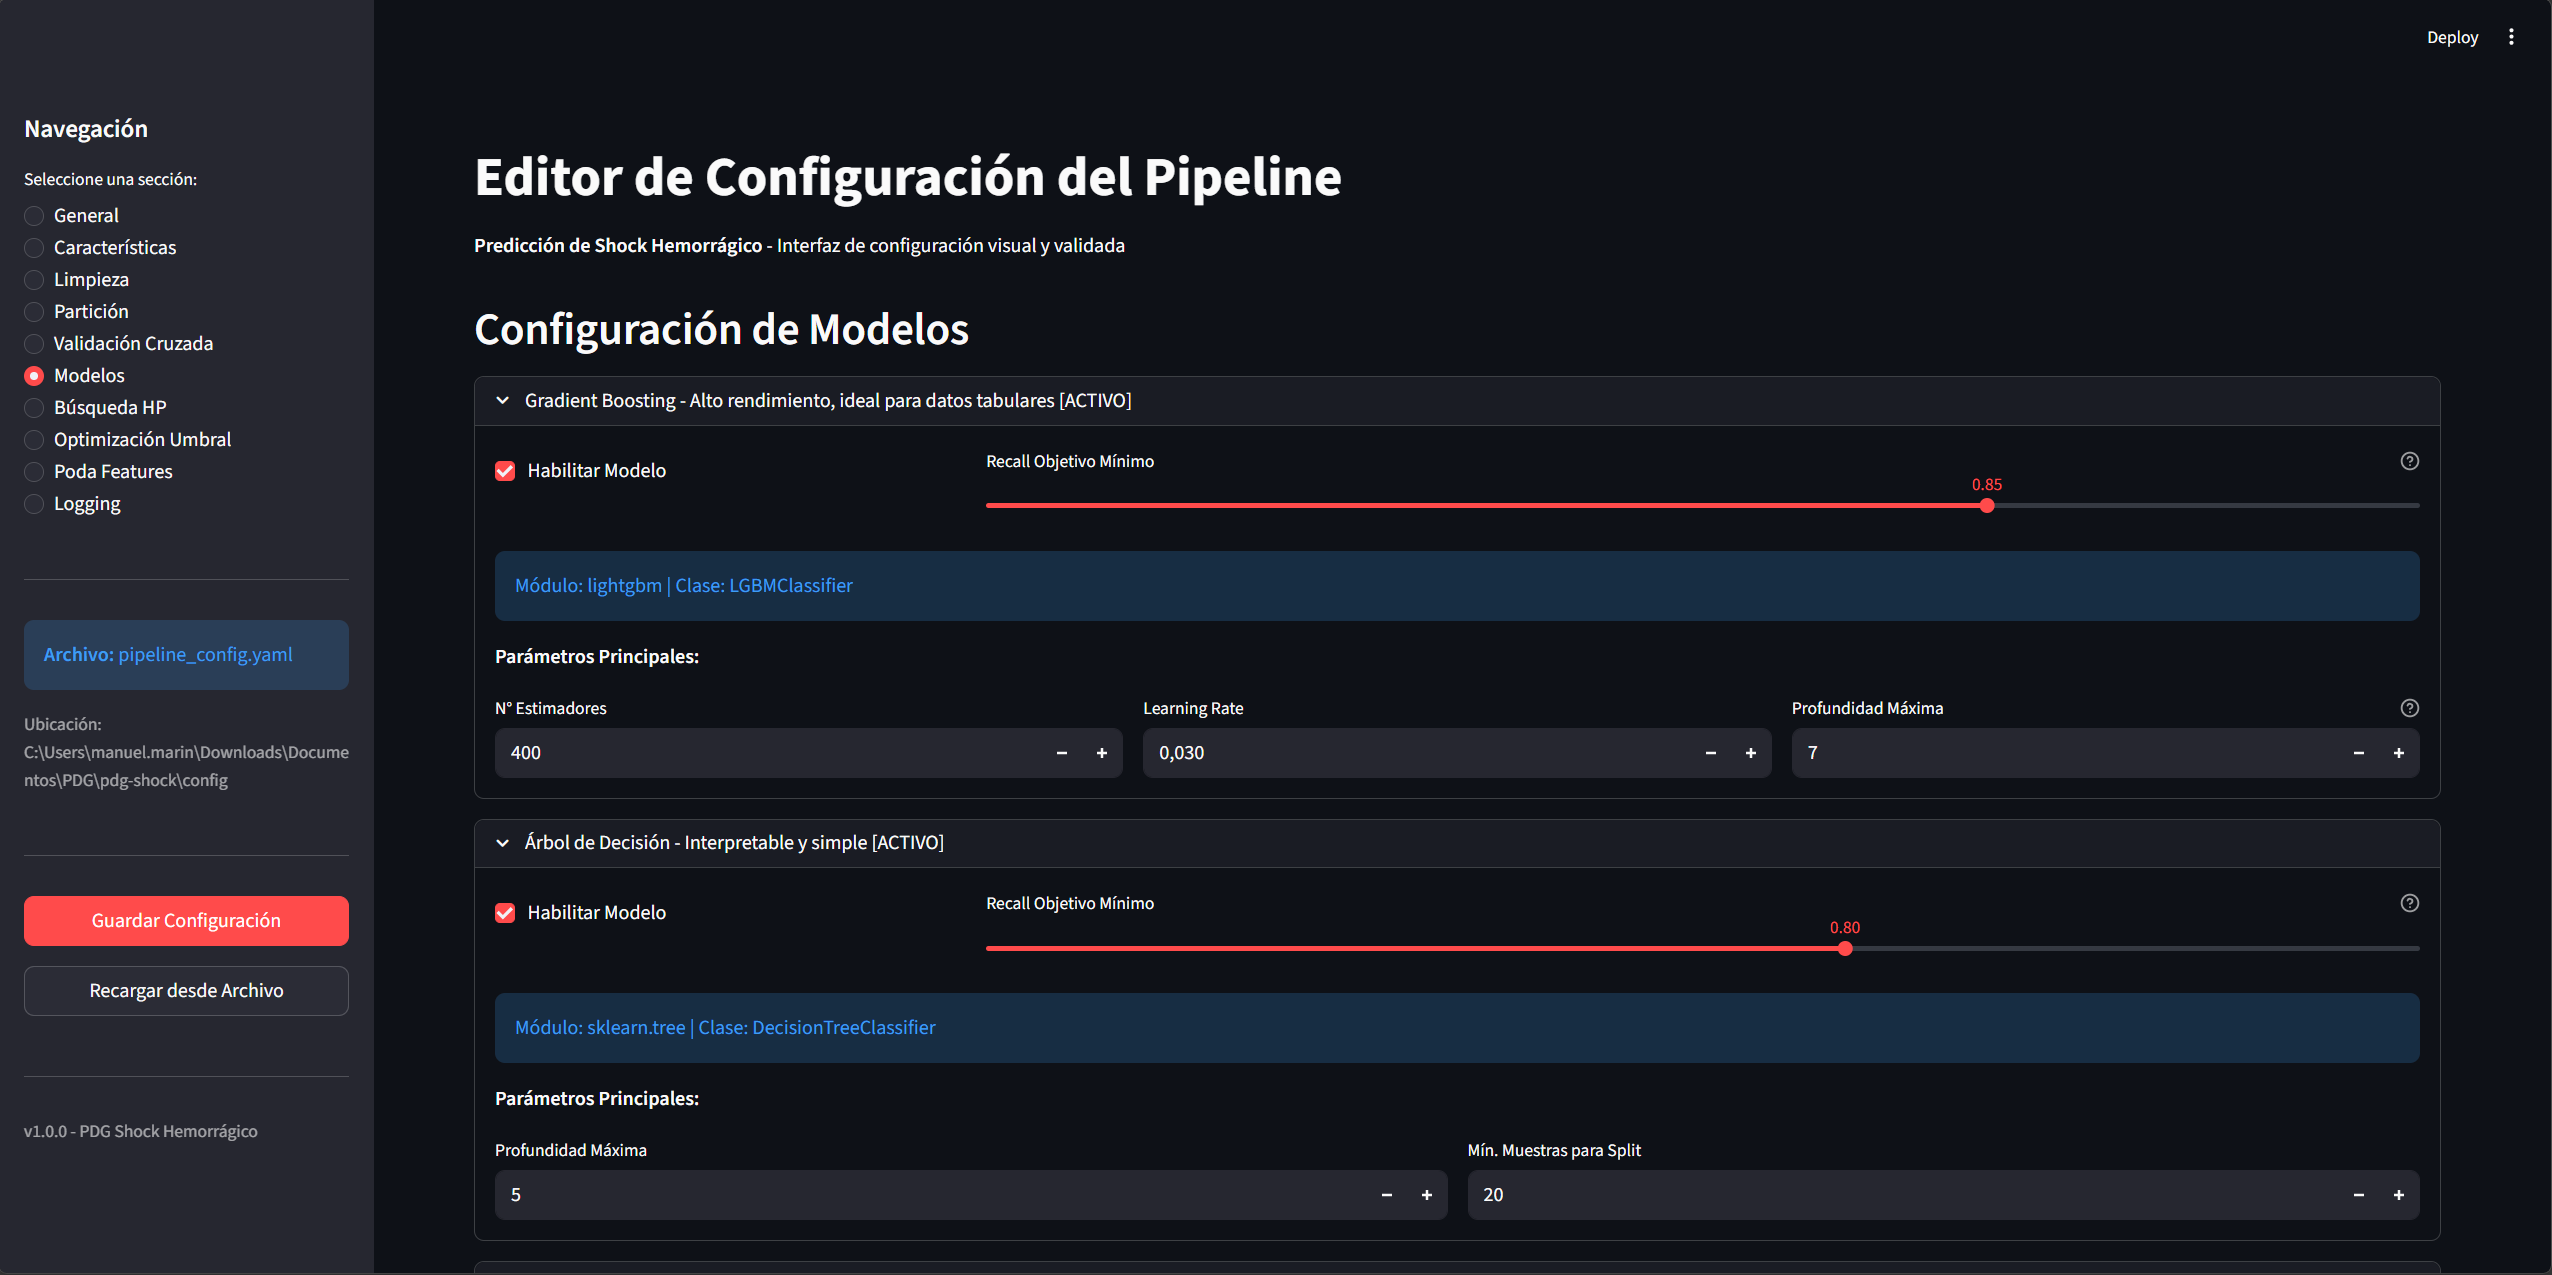
\includegraphics[width=0.85\textwidth]{images/editor_modelos.png}
\caption{Sección de configuración de modelos. Permite habilitar/deshabilitar algoritmos, ajustar hiperparámetros y definir el recall objetivo mínimo.}
\label{fig:editor-modelos}
\end{figure}

La \textbf{sección de configuración de modelos} constituye el núcleo de la experimentación (Figura \ref{fig:editor-modelos}). Para cada algoritmo disponible (LightGBM, Decision Tree, Regresión Logística, Naive Bayes), el usuario puede activar o desactivar su inclusión en el experimento. Cuando un modelo está habilitado, se revela una interfaz de configuración que permite ajustar sus hiperparámetros específicos: número de estimadores, learning rate y profundidad máxima para LightGBM; profundidad máxima y mínimo de muestras para split para Decision Tree; parámetro de regularización C y tipo de penalización (L1, L2, elasticnet) para Regresión Logística. Adicionalmente, se define un umbral de recall objetivo mínimo (por defecto 0.80, no menor a 0.50) que guía la optimización del modelo en el contexto clínico. Este umbral refleja la prioridad de detectar la mayoría de casos de shock verdadero, incluso a costa de falsas alarmas.

La \textbf{sección de búsqueda de hiperparámetros} permite activar y configurar la optimización automatizada de hiperparámetros mediante técnicas como Grid Search o Random Search. Los parámetros configurables incluyen: número de iteraciones (combinaciones a probar), folds para validación cruzada durante la búsqueda y métrica de optimización (F1, F2, recall, precision, ROC-AUC). El sistema advierte al investigador que la búsqueda de hiperparámetros incrementa significativamente el tiempo de entrenamiento. La métrica F2 se destaca como prioritaria para contextos médicos, dado que penaliza más los falsos negativos que los falsos positivos.

La \textbf{sección de optimización de umbral} gestiona el punto de corte para clasificación binaria. El investigador puede definir el rango de búsqueda del umbral óptimo (valores mínimo, máximo y paso) y especificar umbrales a comparar en el conjunto de prueba. Adicionalmente, se configura el número de permutaciones para el test de significancia estadística del AUC-ROC, permitiendo evaluar si las diferencias entre modelos son estadísticamente significativas. El umbral determina a partir de qué probabilidad el modelo clasifica un caso como shock positivo; un umbral bajo incrementa la sensibilidad pero reduce la especificidad.

La \textbf{sección de poda de características} permite eliminar features binarias con baja prevalencia en el dataset. El investigador define el número mínimo de casos positivos (unos) que una variable debe tener para ser incluida en el modelo. Esta funcionalidad automatiza la eliminación de características que, por su rareza, no aportan señal predictiva suficiente y solo introducen ruido. El threshold por defecto es 10 casos, aunque puede ajustarse según las necesidades del experimento.

La \textbf{sección de configuración de logs} gestiona el sistema de registro del pipeline. Permite seleccionar el nivel de log (DEBUG, INFO, WARNING, ERROR, CRITICAL), siendo INFO el nivel recomendado para ejecución normal. También define el directorio donde se almacenarán los archivos de log, facilitando la auditoría y el diagnóstico de errores durante la ejecución del pipeline.

El flujo de trabajo del usuario con la interfaz es el siguiente: (1) el investigador selecciona la sección deseada en la barra lateral; (2) modifica los parámetros según las necesidades del experimento; (3) guarda la configuración mediante el botón correspondiente; (4) el sistema genera automáticamente el archivo YAML con validación de formato, creando previamente un backup de la configuración anterior; (5) el pipeline puede ejecutarse con la nueva configuración, produciendo resultados organizados automáticamente en la estructura de carpetas predefinida. Adicionalmente, el usuario puede recargar la configuración desde el archivo en cualquier momento, revertiendo cambios no deseados.

Esta integración disminuye el riesgo de errores técnicos y hace el sistema más accesible, permitiendo que investigadores de sectores como la medicina puedan establecer y probar configuraciones predictivas de forma más natural e intuitiva, sin necesidad de editar archivos YAML manualmente. La interfaz actúa como una capa de abstracción que aísla la complejidad técnica del pipeline, democratizando el acceso a la experimentación algorítmica.

\newpage

% -----------------------------------------------------------------------------
% 6. CONCLUSIONES
% -----------------------------------------------------------------------------